%Autor: José Luis Huanuqueño Murillo (20170294@lamolina.edu.pe)
\documentclass[12pt,oneside,a4paper]{book}
\usepackage[utf8]{inputenc}
\usepackage[T1]{fontenc}
\usepackage[english]{babel} 
\usepackage[margin=2.5cm]{geometry}
\usepackage[intoc, spanish]{nomencl}
\renewcommand{\nomname}{NOMENCLATURA}
\makenomenclature
\usepackage{etoolbox}
\usepackage{mathptmx}
\usepackage{fancyhdr}
\usepackage{amsmath,amsfonts,amssymb} 
\usepackage{caption} 
\usepackage{setspace}
\usepackage{graphicx} 
\usepackage{csquotes}
\usepackage{changepage}
\usepackage{subcaption}	% Para subfiguras
\usepackage{makeidx}
\usepackage{multirow}
\usepackage{array} 
\usepackage{float}
\usepackage{pdflscape} % Página horizontal
\usepackage{lscape} % Hoja horizontal
\usepackage{pdfpages}
\usepackage{wallpaper}
\usepackage{acronym}
\usepackage{tikz}% Para desarrollar funciones
\usepackage{url} % Para insertar url sin problemas
\usepackage{color} % Para texto con diferente colores
\usepackage{tablefootnote} 
\usepackage{lipsum}
\usepackage{enumitem}
\captionsetup[table]{labelfont=bf,textfont=bf,skip=6pt}
% \captionsetup[figure]{labelfont=bf,textfont=bf}
\captionsetup[figure]{labelfont=bf,skip=10pt,textfont=bf}
\usepackage[font=small,labelfont=bf,width=\textwidth,
justification=centering]{caption}
\setlength{\leftmargini}{1em}
\usepackage{appendix}
\newcommand\listappendixname{ÍNDICE DE ANEXOS}
\newcommand\appcaption[1]{%
  \addcontentsline{app}{section}{#1}}
\makeatletter
\newcommand\listofappendices{%
% \setlength{\parskip}{0.2em} 
  \chapter*{\listappendixname}\@starttoc{app}}
\makeatother
\usepackage{titlesec}
\titleformat{\chapter}[block]
{\vspace{-0.56cm}
{\fontsize{14pt}{ \baselineskip}\selectfont}\bfseries\centering}
{\thechapter}{1em}{\vspace{-1.3cm}}
\titleformat{\section}[block]
{\vspace{0cm}
{\fontsize{12pt}{ \baselineskip}\selectfont}\bfseries}
{\thesection}{1em}{\vspace{-0.4cm}}
\titleformat{\subsection}[block]
{\vspace{-0.6cm}
{\fontsize{12pt}{ \baselineskip}\selectfont}\bfseries}
{\thesubsection}{1em}{\vspace{-0.4cm}}
\titleformat{\subsubsection}[block]
{\vspace{-0.6cm}
{\fontsize{12pt}{ \baselineskip}\selectfont}\bfseries}
{\thesubsubsection}{1em}{\vspace{-0.3cm}}

\renewcommand{\thesection}{\arabic{chapter}.\arabic{section}}
\renewcommand{\thechapter}{\Roman{chapter}.}
\AtBeginDocument{
\renewcommand{\contentsname}{ÍNDICE GENERAL}
\renewcommand{\listtablename}{ÍNDICE DE TABLAS}
\renewcommand{\listfigurename}{ÍNDICE DE FIGURAS}
% \renewcommand{\contentsname}{Lista de Contenidos}
% \renewcommand{\refname}{VIII. REFERENCIAS}
\renewcommand{\figurename}{Figura}
\renewcommand{\tablename}{Tabla}
\renewcommand{\thefigure}{\arabic{chapter}.\arabic{figure}}
\renewcommand{\thetable}{\arabic{chapter}.\arabic{table}}
\renewcommand{\theequation}{\arabic{chapter}.\arabic{equation}}
} % Poner nombre a la Tabla
\setcounter{secnumdepth}{6}% para añadir párrafos y subpárrafos
\setcounter{tocdepth}{5}%para que salgan en la tabla de contenidos los párrafos y subpárrafos

\usepackage[backend=biber,style=apa,citestyle = apa, sorting = nyt]{biblatex}
\addbibresource{References/References.bib}

\usepackage[hidelinks]{hyperref}
\usepackage[flushleft]{threeparttable}
\usepackage{booktabs}
\renewcommand{\headrulewidth}{0pt}
\renewcommand{\baselinestretch}{1.5}

\doublespacing
\begin{document}

\frontmatter

\newgeometry{top=3.5cm, bottom= 2.5cm, right=2.5cm, left=2.5cm}
\begin{titlepage}
\centering
 {\fontsize{18pt}{ \baselineskip}\selectfont \textbf{UNIVERSIDAD NACIONAL AGRARIA LA MOLINA}}\\[0.25cm]
 {\fontsize{16pt}{ \baselineskip}\selectfont \textbf{FACULTAD DE INGENIERÍA AGRÍCOLA}}\\[1cm]
\begin{figure}[htb]
\centering

\includegraphics[width=4.5cm, height=5cm]{Cover/Escudo_UNALM.pdf}
\end{figure}
\vspace{0.5cm}
{\fontsize{14pt}{ \baselineskip}\selectfont \textbf{PROYECTO DE TESIS:}}\\[0.5cm]
{\fontsize{14pt}{ \baselineskip}\selectfont \textbf{``TÍTULO''}}\\[0.5cm]
{\fontsize{14pt}{ \baselineskip}\selectfont \textbf{AUTOR:}}\\[0.5cm]
{\fontsize{14pt}{ \baselineskip}\selectfont \textbf{NOMBRE DEL AUTOR}}\\[0.5cm]
{\fontsize{14pt}{ \baselineskip}\selectfont \textbf{ASESOR:}}\\[0.5cm]
{\fontsize{14pt}{ \baselineskip}\selectfont \textbf{NOMBRE DEL ASESOR}}\\[0.5cm]
% \large{\textbf{LIMA-PERÚ \\ 2020}}
\vfill
{\fontsize{14pt}{ \baselineskip}\selectfont \textbf{LIMA - PERÚ}}\\[0.5cm]
{\fontsize{14pt}{ \baselineskip}\selectfont \textbf{2021}}
\singlespacing
\rule{132mm}{0.25mm}\\
{\small \textbf{La UNALM es titular de los derechos patrimoniales de la presente investigación\\ (Art.24 - Reglamento de propiedad intelectual)}}
\end{titlepage}
\restoregeometry
% \newgeometry{margin= 2.5cm} 

\pagenumbering{roman}

\begin{center}
\thispagestyle{empty}
 {\fontsize{18pt}{ \baselineskip}\selectfont \textbf{UNIVERSIDAD NACIONAL AGRARIA LA MOLINA}}\\[0.25cm]
 {\fontsize{16pt}{ \baselineskip}\selectfont \textbf{FACULTAD DE INGENIERÍA AGRÍCOLA}}\\[1cm]
 {\fontsize{16pt}{ \baselineskip}\selectfont \textbf{``TÍTULO''}}\\[0.5cm]
 {\fontsize{16pt}{ \baselineskip}\selectfont TESIS PARA OPTAR EL TÍTULO PROFESIONAL DE:}\\[0.5cm]
 {\fontsize{16pt}{ \baselineskip}\selectfont\textbf{INGENIERO AGRÍCOLA}}\\[0.5cm]
 {\fontsize{14pt}{ \baselineskip}\selectfont Presentado por:} \\[0.5cm]
 {\fontsize{16pt}{ \baselineskip}\selectfont \textbf{BACH. ...}}\\[0.5cm]
 {\fontsize{14pt}{ \baselineskip}\selectfont Sustentado y aprobado por el siguiente jurado:}\\[1cm]
\begin{minipage}{\linewidth}
\centering
\singlespacing
\begin{tabular}{cc}
\hrulefill & \hrulefill \\
 {\fontsize{10pt}{ \baselineskip}\selectfont{Dr. ...}} &  {\fontsize{10pt}{ \baselineskip}\selectfont Dr. Mg. Sc. Ing. ...} \\
\small{\textbf{Presidente}} & \small{\textbf{Asesora}}
\end{tabular}\\[1cm]
\begin{tabular}{cc}
\hrulefill & \hrulefill \\
{\fontsize{10pt}{ \baselineskip}\selectfont{Mg. Sc. ...}} & {\fontsize{10pt}{ \baselineskip}\selectfont{Mg. Sc. ...}} \\
\small{\textbf{Miembro}} & \small{\textbf{Miembro}}
\end{tabular}\\[1cm]
\begin{tabular}{c}
\hrulefill \\
{\fontsize{10pt}{ \baselineskip}\selectfont{Ing. ...}} \\
\small{\textbf{Co-Asesor}} 
\end{tabular}
\end{minipage}
\vfill
{\fontsize{14pt}{ \baselineskip}\selectfont \textbf{LIMA - PERÚ}}\\[0.5cm]
{\fontsize{14pt}{ \baselineskip}\selectfont \textbf{2021}}
\singlespacing
\end{center}
\addcontentsline{toc}{chapter}{\textbf{PORTADA}}

\newgeometry{top=7cm, bottom= 4cm, right=2.5cm, left=6cm}
\chapter*{\hfill DEDICATORIA}
\thispagestyle{empty}
\doublespacing
\begin{flushright}
\textit{Dedicado a tada mi familia, en especial a mis padres y papitos, mamá Teodora y papá Murillo, gran parte de mi infancia viví con ellos y siempre los tendré presente en mi corazón. También a esa persona que tanto me ha ayudado emocionalmente e intelectualmente.}
\end{flushright}


\addcontentsline{toc}{chapter}{\textbf{DEDICATORIA}}
\restoregeometry
\chapter*{\flushright AGRADECIMIENTO}
\doublespacing
\begin{flushright}
       A mis profesores, compañeros, amigos, padres, novia, etc
\end{flushright}

\addcontentsline{toc}{chapter}{\textbf{AGRADECIMIENTO}}

\doublespacing
\tableofcontents
\addcontentsline{toc}{chapter}{\textbf{ÍNDICE GENERAL}}
\pagestyle{fancy}
\fancyhf{}
\fancyfoot[c]{\thepage}
\listoftables
\addcontentsline{toc}{chapter}{\textbf{ÍNDICE DE TABLAS}}
\listoffigures
\addcontentsline{toc}{chapter}{\textbf{ÍNDICE DE FIGURAS}}
\listofappendices
\addcontentsline{toc}{chapter}{\textbf{ÍNDICE DE ANEXOS}}

\doublespacing
\setlength{\parskip}{1em} 
\setlength{\parindent}{0cm}
% \clearpage
\onehalfspacing
\mbox{}

\nomenclature{VANT}{Vehículo Aéreo No Tripulado}
\nomenclature{SEBAL}{Algoritmo de balance de energía superficial para tierra}
\nomenclature{SEB}{Componentes del balance de energía}
\nomenclature{METRIC}{Mapeo de la evapotranspiración a alta resolución con calibración internalizada}
\nomenclature{METRIC-HR}{METRIC de alta resolución}
\nomenclature{DTD}{Diferencia de temperatura dual}
\nomenclature{ANN}{Neuronales artificiales}
\nomenclature{ML}{Machine learning}
\nomenclature{DL}{Deep learning}
\nomenclature{RSEB}{Balance energético con información de teledetección}
\nomenclature{IAF}{Índice de área foliar}
\nomenclature{SAVI}{Índice de vegetación ajustado al suelo}
\nomenclature{NDVI}{Índice de Vegetación de Diferencia Normalizada}
\nomenclature{BRDF}{Función de distribución de reflectancia bidireccional}
\nomenclature{NDVIc}{Índice de Vegetación de Diferencia Normalizada para el canopy}
\nomenclature{NDVIss}{Índice de Vegetación de Diferencia Normalizada para el suelo}
\nomenclature{TSEB}{Balance de energía de dos fuentes}
\nomenclature{STSEB}{Salance energético simplificado existente de dos fuentes}
\nomenclature{ET}{Evapotranspiración}
\nomenclature{ET}{Evapotranspiración}
\nomenclature{ETo}{Evapotranspiración de referencia}
\nomenclature{Etc}{Evapotranspiración real o del cultivo}
\nomenclature{G}{Flujo de calor del suelo}
\nomenclature{H}{Flujo de calor sensible}
\nomenclature{$\mathrm{R_{n}}$}{Radiación neta}
\nomenclature{$R_{s}$}{Radiación de onda corta entrante}
\nomenclature{$R_{l}$}{Radiación de onda larga entrante}
\nomenclature{LE}{Flujo de calor latente}
\nomenclature{$LE_{v}$}{Transpiración del dosel}
\nomenclature{$LE_{s}$}{Evaporación del agua del suelo}

\printnomenclature[1in]
\doublespacing
\setlength{\parindent}{0cm}
\setlength{\parskip}{1em} 
\chapter*{RESUMEN}
\lipsum[1]

\lipsum[2]\\\vspace{1em}

\textbf{Palabras claves:} Zonificación Agroecológica, Duraznero, Proceso Analítico Jerarquizado, Sistemas de Información Geográfica, San Pablo de Pillao, Sequías.
\addcontentsline{toc}{chapter}{\textbf{RESUMEN}}

\chapter*{ABSTRACT}

\lipsum[1]

\lipsum[2]\\\vspace{1em}

\textbf{Key Words:} Agroecological Zoning, Peach, Hierarchical Analytical Process, Geographic Information Systems, San Pablo de Pillao, Droughts.
\addcontentsline{toc}{chapter}{\textbf{ABSTRACT}}

\newpage
\doublespacing
\mainmatter
\pagestyle{fancy}
\fancyhf{}
\fancyfoot[c]{\thepage}

% \setlength{\parskip}{\baselineskip} 
\setlength{\parindent}{0cm}
\setlength{\parskip}{1em} 

\chapter{INTRODUCCIÓN}
\thispagestyle{empty}
\lipsum[1]

\lipsum[2]\nocite{*}


% % \chapter{OBJETIVOS}
% \thispagestyle{empty}
% \section{Objetivos generales}
% Caracterizar los recursos hídricos e identificar las zonas vulnerables en el ámbito del Proyecto Especial Tambo Ccaracocha mediante el modelamiento geoespacial y presentar alternativas de aprovechamiento de los recursos hídricos.

% \section{Objetivos específicos}
% % [leftmargin=1em]
% \begin{itemize}
%     \item Determinar la oferta y demanda hídrica en el ámbito de influencia del Proyecto Especial Tambo-Ccaracocha. 
%     \item Presentar alternativas de proyectos, para contribuir a la segurar el afianzamiento hídrico para el valle de Ica. 
%     \item Generar una base de datos geoespacial, para caracterizar e identificar el grado de vulnerabilidad en el ámbito del Proyecto Tambo Ccaracocha.
%     \item Desarrollar el modelo geoespacial para identificación del grado de vulnerabilidad en el ámbito del Proyecto. 
% \end{itemize}



\chapter{REVISIÓN DE LITERATURA}
\thispagestyle{empty}
\section{Balance de Energía para Estimar la ET a partir de Imágenes de Satélite }

\lipsum[1]

\lipsum[2]

\section{Balance de energía para estimar la ET a partir de imágenes de un VANT}

\lipsum[1]

\lipsum[2]

\subsection{SEBAL}

\lipsum[1]

\lipsum[2] \parencite{Lee2016}.

En la Figura 1 se observa los pasos a seguir en el procesamiento de las imágenes de satélite según el algoritmo SEBAL y modificacion propuesta por \parencite{Lee2016}. 

\lipsum[3] \parencite{Lee2016}.

\begin{equation}
   \mathrm{ \lambda  ET = R_{n} - G - h}
\end{equation}
donde $\lambda ET$ es el flujo de calor latente ($w\times m^{-2}$), $R_{n}$ es la radiación neta en la superficie ($w\times m^{-2}$), $G$ es el flujo de calor del suelo ($w\times m^{-2}$), y $h$ es el flujo de calor sensible al aire ($w\times m^{-2}$). La evapotranspiración se calcula utilizando la siguiente ecuación $\left [\lambda ET\times \left ( R_{n} - G \right )^{-1} \right]$.

\begin{figure}[htbp!]
    \centering
    
\includegraphics[width=0.3\textwidth]{Cover/Escudo_UNALM.pdf}
    \caption{UNALM}
    \captionsetup{labelfont=rm,skip=2pt,textfont=rm,font=small}
        \caption*{\textbf{FUENTE:} \parencite{Lee2016}}
    \label{fig:1}
\end{figure}

Al aplicar el modelo SEBAL, es importante la selección de dos píxeles ``ancla'' (píxel ``caliente" y ``frío") sobre el área de interés, que se utilizan para determinar las diferencias de temperatura entre la temperatura de la superficie ($T_{s}$) y la temperatura del aire ($dT$). Se supone que existe una relación lineal entre $T_{s}$ y $dT$ en forma de:
\begin{equation}
    dT = aT_{s} + b
\end{equation}
donde a y b son las constantes de relación lineal. Para determinar estas constantes, SEBAL utiliza los dos píxeles ``ancla" para los cuales se puede estimar confiablemente un valor para h. $T_{s}$ se estima a partir de la temperatura de la superficie terrestre (LST)  para cada píxel; $dT$ se calcula para el píxel ``caliente" o ``frío" utilizando la siguiente relación:
\begin{equation}
    dT_{\frac{cold}{hot}} = h_{\frac{cold}{hot}}{r_{ah}}_{\frac{cold}{hot}}/\left ( \rho_{\frac{cold}{hot}}c_{p} \right )
\end{equation}
donde h puede calcularse para los píxeles de anclaje utilizando datos meteorológicos, $\rho$  es la densidad del aire ($kg\times m^{-3}$), $Cp$ es el calor específico del aire ($1004 J\times kgK^{-1}$), $dT$ es la diferencia de temperatura entre dos alturas ($K$), y rah es la resistencia aerodinámica al transporte de calor ($s\times m^{-1}$) para cada píxel ``frío" y ``caliente". La anterior relación lineal entre $dT$ y $T_{s}$ es una presunción importante en el SEBAL.

El píxel frío se utiliza para definir la cantidad de evapotranspiración. Para identificar los píxeles fríos en la zona de interés se suele utilizar un cultivo o una masa de agua que cubra toda la superficie. Sin embargo, la temperatura de la superficie que se utiliza debe ajustarse uniformemente a una elevación de referencia común para una predicción precisa de $dT$. De lo contrario, las altas elevaciones que parecen ``frías" pueden interpretarse erróneamente como que tienen una alta evaporación. Por ello se procede a realizar una corrección de la temperatura. En el procedimiento se utilizaron los datos del MED para este cálculo. La temperatura superficial corregida por el MED es calculada por la siguiente ecuación:
\begin{equation}
    T_{0_{-}dem} = T_{0} + 0.0065\Delta z
\end{equation}
donde $\Delta z $ es la diferencia de la elevación de un píxel con respecto al dato ($m$).

A partir del residuo en la ecuación de balance energético instantáneo y la fracción de evaporación ($\Lambda$), se estimó el ET diario ($ET_24$), $mm\times d^{-1}$. $\Lambda$ es notablemente regular y relativamente constante en los días sin nubes. Por lo tanto, su valor instantáneo puede tomarse como el valor medio diario, de modo que la variabilidad espacial en la ET diaria puede predecirse a gran escala.
\begin{equation}
    \Lambda = \frac{\lambda ET}{R_{n} - G}
\end{equation}
\begin{equation}
    ET_{24} = \frac{86500\Lambda \left ( R_{n,24} - G_{24} \right )}{\lambda }
\end{equation}
donde $R_{n,24}$ es la radiación neta diaria; $G_{24}$ es el flujo de calor diario del suelo; 86.400 es el número de segundos en un período de 24 h; y $\Lambda$ es el calor latente de vaporización ($J\times kg^{-1}$). El calor latente de vaporización permite la expresión de $ET_{24}$ en $mm\times d^{-1}$. El parámetro $G_{24}$ puede ser aproximado para las superficies vegetativas y del suelo como cero en la superficie del suelo. Esto se debe a que, en promedio, la energía almacenada en el suelo durante el día se libera en el aire durante la noche. La vaporización de calor latente y $R_{n,24}$ se definen como:
\begin{gather}
     \lambda = \left ( 2.501 - 0.00236\left ( T_{0} - 273 \right )\times 10^{6}  \right ) \left (  J\times kg^{-1}\right ) \\
     R_{n,24} = \left ( 1 - \alpha  \right )Rs_{24} - a\tau _{sw}
\end{gather}
donde $Rs_{24}$ es la radiación solar entrante de 24 horas; alfa es el albedo; a es un coeficiente de regresión de la relación entre la radiación de onda larga neta y la transmisibilidad atmosférica a escala diaria; y $\tau _{sw}$ es la de transmisión unidireccional en un cielo claro y puede predecirse para condiciones atmosféricas claras y relativamente secas utilizando la elevación sobre el nivel del mar en $m$. El coeficiente a puede aplicarse de manera diferente según a la región.

\parencite{Lee2016} estimaron la evapotranspiración espacial diaria utilizando el algoritmo SEBAL modificado con una selección automática mejorada para el píxel de ancla y datos mensuales para mejorar los resultados, utilizando los datos del Terra MODIS para Corea del Sur. Los mismos que constan de  36 canales espectrales discretos con una resolución espacial de 250 m para bandas visibles, 500 m para bandas de infrarrojo cercano y 1000 m para las bandas de infrarrojos térmicos restantes. Los resultados espaciales de la ET obtenidos mediante el modelo SEBAL se validaron utilizando dos años (2012-2013) de datos de ET de torres de flujo medidos en tres lugares (dos en un bosque y uno en un arrozal). 

Para píxeles\footnote{Medida de cada cuadrante del espectro.} fríos, se selecciono el 5\% superior del NDVI más alto y, entre ellos, se selecciono el 15\% más frío de la Ts dentro de un área agrícola del área según el uso de la tierra. Para píxeles calientes, se selecciono el 10\% más bajo del NDVI y luego se selecciono el 15\% más caliente de la Ts dentro de un campo desnudo o un área urbana de acuerdo con el uso de la tierra. Se hace referencia al estándar para los candidatos a píxeles de anclaje, sin embargo, el porcentaje se ajusta ligeramente de 20\% a 15\% porque hay muchos píxeles en el área de interés y puede afectar el tiempo de ejecución total del modelo. Durante el período de este estudio (2012-2013), el valor máximo de la temperatura superficial de la tierra (LST) mostró el rango de aproximadamente 279.2 K a 321.0 K, mientras que el valor mínimo de LST indicó el rango de aproximadamente 252,1 K a 295,4 K. Generalmente, los píxeles calientes se seleccionaron en el rango de 277,1 K a 319,1 K, y los píxeles fríos se incluyeron en el rango de 253,6 K a 296,4 K. El LST fue el factor clave, además de los datos de los satélites, para estimar la variabilidad temporal diaria de la ET \parencite{Lee2016}.

\lipsum[1]

\lipsum[3]

\begin{table}[H]
\centering
\begin{threeparttable}
\caption{Características de la torre de flujo CFK ubicada al centro de arrozales}
\label{tab:1}
\begin{tabular}{@{}lc@{}}
\hline
\multicolumn{1}{c}{Sitio} & Cheongmicheon (CFK) \\ \hline
Latitud (N) & 37$^{\circ}$ 090 35” \\
Longitud (E) & 127$^{\circ}$ 390 10” \\
Elevación (m) & 141 \\
Temperatura media anual ($^{\circ}$C) & 11.5 \\
Precipitación media anual (mm) & 1107 \\
Velocidad del viento media (m/s) & 1.97 \\
Tierra usada & Arrozal \\ \hline
\end{tabular}
    \begin{tablenotes}
    \vspace{-0.5cm}
      \item {{\fontsize{10pt}{ \baselineskip}\selectfont \textbf{FUENTE}: \parencite{Lee2016}}}
    \end{tablenotes}
\end{threeparttable}
\end{table}
\vspace{-0.6cm}
La Figura \ref{fig:2} muestra la variación diurna de los componentes de balance energético sobre la superficie transpirante bien regado en un día despejado en un arrozal. El flujo de calor del suelo se encuentra en el rango de 0 a 100 $W\times m^{-2}$ y el flujo de calor sensible se encuentra en el rango de aproximadamente 50 a 400 $W\times m^{-2}$.

\begin{figure}[H]
    \centering
    
\includegraphics[width=0.4\textwidth]{Cover/Escudo_UNALM.pdf}
    \caption{Variación temporal de los componentes del balance energético en la torre de flujo ubicada al centro de arrozales}
    \captionsetup{labelfont=rm,skip=2pt,textfont=rm,font=small}
        \caption*{\textbf{FUENTE:} \parencite{Lee2016}}
    \label{fig:2}
\end{figure}

En condiciones climáticas casi nubladas, la radiación solar ($Rs$) en lugar de $Ra(24)t(sw)$, mejoró los resultados del r2 del SEBAL en arrozales de 0,52 a 0,77, es decir se debe utilizar un valor medido local (en tierra) para la radiación solar (Rs) de 24 horas en lugar de $Ra(24)\tau (sw)$. Esto depende del porcentaje de nubosidad del lugar de estudio. Ver Figura \ref{fig:3}. 

\begin{figure}[H]
    \centering
    
\includegraphics[width=0.3\textwidth]{Cover/Escudo_UNALM.pdf}
    \caption{UNALM}
    \captionsetup{labelfont=rm,skip=2pt,textfont=rm,font=small}
        \caption*{\textbf{FUENTE:} \parencite{Lee2016}}
    \label{fig:3}
\end{figure}
\vspace{-0.6cm}
La Figura \ref{fig:4} se muestra la ET en arrozales obtenida por \parencite{Lee2016} con ET total de 496,1 y 467,8 mm para el 2012 y 2013 respectivamente (torre de flujo) y 5,2 y 5,3 $mm\times d^{-1}$ según la torre de flujo y SEBAL, respectivamente; con mejor ajuste de la ET para el año 2013 con valores de Indice de Nash de 0.73 y r2 de 0.80.

\begin{figure}[H]
    \centering
    
\includegraphics[width=0.4\textwidth]{Cover/Escudo_UNALM.pdf}
    \caption{UNALM}
    \captionsetup{labelfont=rm,skip=2pt,textfont=rm,font=small}
        \caption*{\textbf{FUENTE:} \parencite{Lee2016}}
    \label{fig:4}
\end{figure}
\vspace{-0.6cm}
La Figura \ref{fig:5} muestra los datos mensuales del NDVI, el albedo y  ET según las torres de flujo. El NDVI de la zona de arrozales muestra el patrón de crecimiento y desarrollo de la planta de mayo a septiembre, el NDVI de las zonas de bosques mixtos muestra un patrón diferente, con valor superior a 0,5 de abril a noviembre. En la temporada de invierno (particularmente en diciembre), el NDVI del bosque tiende a ser más bajo que el de arrozales, esto debido a que está situado a una mayor altitud. Es decir, SEBAL refleja las características geográficas, con  ET en las zonas bajas, mayores que en zonas de mayor altitud.

\begin{figure}[H]
    \centering
    
\includegraphics[width=0.4\textwidth]{Cover/Escudo_UNALM.pdf}
    \caption{UNALM}
    \captionsetup{labelfont=rm,skip=2pt,textfont=rm,font=small}
        \caption*{\textbf{FUENTE:} \parencite{Lee2016}}
    \label{fig:5}
\end{figure}
\vspace{-0.6cm}
\lipsum[3]

\lipsum[2]

\subsection{METRIC}

\lipsum[1]

\lipsum[2]

\parencite{Bhattarai2017} estimaron la ET en tres sitios del USA con sitios de flujo EC en FL y un sitio llamado Ameriflux, Medición de la Radiación Atmosférica en las Grandes Llanuras del Sur (ARM SGP), en OKLAHOMA (OK), informacion que se utilizaron para demostrar el modelo automatizado desarrollado en este estudio.  La estación de Blue Cypress cubre un gran sistema de humedales de llanura de inundación en la cabecera del río St. Johns en el condado de Indian River en el centro-oeste. El sitio de Citrus cubre una arboleda de 22 ha de cítricos de bosque plano. La Ferris está situado en zona de pastos (Paspalum notatum) y los campos de fresas. El sitio ARM-SGP es una gran estación agrícola experimental (periódica rotación del trigo, el maíz y la soja) con un clima más seco.

\subsubsection{Los datos medidos de la ET}

\lipsum[4]

\begin{table}[H]
\centering
\begin{threeparttable}
\caption{Descripción de los sitios utilizados en este estudio}
\label{tab:2}
\begin{tabular}{@{}lc@{}}
\hline
\multicolumn{1}{c}{Descripciones del sitio} & ARM SGP \\ \hline
Latitud ($^{\circ}$N) & 36.6058 \\
Longitud ($^{\circ}$W) & 97.4888 \\
Tipo de cobertura & Cultivos \\
Periodo de medición de la ET$^{a}$ & 2000-2015 \\
Tiempo medio anual ($^{\circ}$C) & 15 \\
Precipitación media anual (mm) & 383 \\
La media diaria de la ET (mm dia) & 1.3 \\
Altura del dosel (m) & Variante \\
Altura de la torre (m) & 60 \\
Fuente para más información & ARM Climate Research Facility \\ \hline
\end{tabular}
    \begin{tablenotes}
    \vspace{-0.5cm}
      \item {{\fontsize{10pt}{ \baselineskip}\selectfont \textbf{FUENTE}: \parencite{Bhattarai2017}}}
    \end{tablenotes}
\end{threeparttable}
\end{table}
\vspace{-0.6cm}
Diseñamos específicamente nuestro algoritmo de automatización para trabajar con imágenes térmicas de Landsat. El tamaño de 30 m de píxeles - la banda térmica es remuestreada a 30 m para igualar las bandas multiespectrales. Landsat permite el mapeo de la ET a escalas de campo, por lo que los datos de Landsat son ampliamente utilizados en la gestión de los recursos hídricos.  Las imágenes Landsat de La superficie se procesaron por el Sistema de Procesamiento Adaptativo de Perturbaciones (LEDAPS) reflectancia (Masek et al., 2006) (bandas 1-5 y 7), la imagen termal Landsat y los metadatos de la imagen se obtuvieron del USGS (\url{www.glovis.usgs.gov} y \url{http://landsat.usgs.gov/lsrd_sw.php}; último acceso 06/10/2015). Las ortoimágenes a nivel estatal con un tamaño de 1 m de píxel se obtuvieron del Departamento de Agricultura de los Estados Unidos (USDA).

\subsubsection{Las datos Meteorológicos}

Datos meteorológicos de intervalo temporal de 15 minutos disponibles gratuitamente desde la plataforma de la Red Meteorológica Automatizada de la Florida (FAWN) (Figura 6; \url{http://fawn.ifas.ufl.edu/ about_index.php} y Oklahoma Mesonet  \url{https://www.mesonet.org/} se utilizaron en este estudio. Un mapa ráster para cada estación instantánea y los parámetros meteorológicos diarios (es decir, velocidad del viento, temperatura, la radiación solar, y la humedad relativa).

\subsubsection{Datos de la Cubierta Terrestre}

Datos disponibles de 30 m de cobertura terrestre del USGS National Land Cover Base de datos (NLCD; \url{http://www.mrlc.gov/index.php}) se utilizaron para identificar las tierras agrícolas tanto para el manual como para  los enfoques automatizados de selección de píxeles de los miembros.  Las tierras agrícolas incluían ambos cultivos y los pastos. Las descripciones e implementación de los modelos SEBAL y MÉTRIC, se basan en que la ET puede ser estimada a partir del término residual del balance energético de la superficie ecuación (Ec. (1)). Rn se calcula para las condiciones de cielo despejado (Ec. (9)) G se calcula como la fracción de Rn (Ec. (10)).

\begin{table}[H]
\centering
\begin{threeparttable}
\caption[Estaciones meteorológicas]{\textbf{Estaciones meteorológicas}}
\label{tab:my-tablez}
\begin{tabular}{@{}lcccc@{}}
\hline
Estaciones & Este (m) & Norte (m) & Latitud & Longitud \\ \hline
Tunel cero & 490680.81 & 8534186.15 & 13$^{\circ}$15'33.54'' & 75$^{\circ}$5'8'' \\
Ocucaje & 426464.86 & 8410316.41 & 14$^{\circ}$22'42.2'' & 75$^{\circ}$40'0'' \\ \hline
\end{tabular}
    \begin{tablenotes}
    \vspace{-0.5cm}
      \item {{\fontsize{10pt}{ \baselineskip}\selectfont \textbf{FUENTE}: Elaboración propia}}
    \end{tablenotes}
\end{threeparttable}
\end{table}

\newpage
\begin{landscape}
\pagestyle{empty}
\begin{figure}
    \centering
    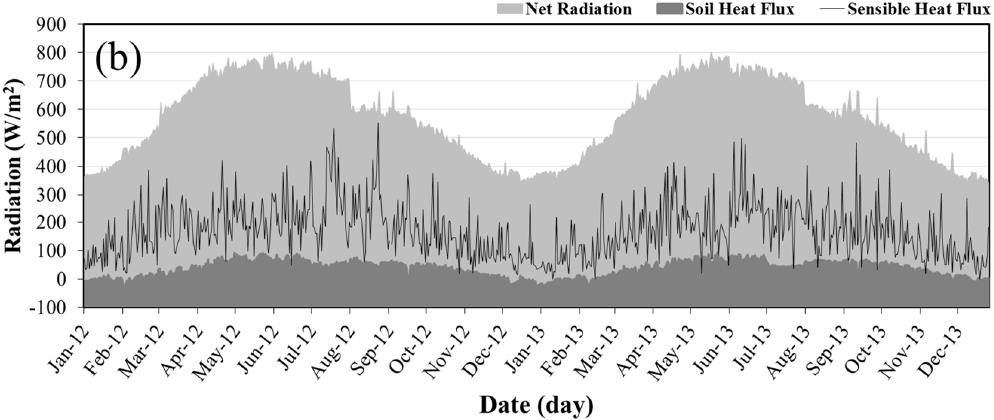
\includegraphics[width=1\textwidth]{Figures/f2.png}
    \caption{Diagrama de modelos}
    \label{fig:my_label5}
\end{figure}
\end{landscape}




\chapter{METODOLOGÍA}
\thispagestyle{empty}

\begin{itemize}[leftmargin=1em]
    \item La siguiente Tabla \ref{tab:my-table1} es de clasificación de suelos:
\end{itemize}
\begin{table}[H]
\centering
\begin{threeparttable}
\caption[Clasificación de suelos]{Clasificación de suelos para determinarlo en el laboratorio del departamento de ordenamiento territorial}
\label{tab:my-table1}
\begin{tabular}{@{}ccccc@{}}
\hline
\multicolumn{1}{c}{} &
  \multicolumn{1}{c}{BRITÁNICO} &
  \multicolumn{1}{c}{AASHTO} &
  \multicolumn{1}{c}{ASTM} &
  \multicolumn{1}{c}{SUCS} \\ \cline{2-5} 
\multicolumn{1}{c}{\multirow{-2}{*}{SISTEMAS}} &
  \multicolumn{1}{c}{{\color[HTML]{4D5156} (mm)}} &
  \multicolumn{1}{c}{{\color[HTML]{4D5156} (mm)}} &
  \multicolumn{1}{c}{{\color[HTML]{4D5156} (mm)}} &
  \multicolumn{1}{c}{{\color[HTML]{4D5156} (mm)}} \\ \hline
\multicolumn{1}{c}{Grava} &
  \multicolumn{1}{c}{60 - 2} &
  \multicolumn{1}{c}{75 - 2} &
  \multicolumn{1}{c}{\textgreater 2} &
  \multicolumn{1}{c}{75 - 4,75} \\ \hline
\multicolumn{1}{c}{Arena} &
  \multicolumn{1}{c}{2 - 0,006} &
  \multicolumn{1}{c}{2 - 0,05} &
  \multicolumn{1}{c}{2 - 0,075} &
  \multicolumn{1}{c}{4,75 - 0,075} \\ \hline
\multicolumn{1}{c}{Limo} &
  \multicolumn{1}{c}{0,06 - 0,002} &
  \multicolumn{1}{c}{0,05 - 0,002} &
  \multicolumn{1}{c}{0,075 - 0,005} &
  \multicolumn{1}{c}{\textless 0,075 FINOS} \\ \hline
\multicolumn{1}{c}{Arcilla} &
  \multicolumn{1}{c}{\textless  0,002} &
  \multicolumn{1}{c}{\textless  0,002} &
  \multicolumn{1}{c}{\textless  0,005} &
  \multicolumn{1}{c}{} \\ \hline
\end{tabular}
    \begin{tablenotes}
    \vspace{-0.5cm}
      \item {{\fontsize{10pt}{ \baselineskip}\selectfont \textbf{FUENTE}: Elaboración propia}}
    \end{tablenotes}
\end{threeparttable}
\end{table}


\begin{table}[H]
\centering
\begin{threeparttable}
\caption[Estaciones meteorológicas]{\textbf{Estaciones meteorológicas}}
\label{tab:my-table}
\begin{tabular}{@{}lcccc@{}}
\hline
Estaciones & Este (m) & Norte (m) & Latitud & Longitud \\ \hline
Tunel cero & 490680.81 & 8534186.15 & 13$^{\circ}$15'33.54'' & 75$^{\circ}$5'8'' \\
Ocucaje & 426464.86 & 8410316.41 & 14$^{\circ}$22'42.2'' & 75$^{\circ}$40'0'' \\ \hline
\end{tabular}
    \begin{tablenotes}
    \vspace{-0.5cm}
      \item {{\fontsize{10pt}{ \baselineskip}\selectfont \textbf{FUENTE}: Elaboración propia}}
    \end{tablenotes}
\end{threeparttable}
\end{table}

\begin{table}[H]
\centering
  \begin{threeparttable}
\caption{Estaciones meteorológicas}
\label{tab:my-table2}
\begin{tabular}{@{}lcccc@{}}
\hline
Estaciones & Este (m) & Norte (m) & Latitud & Longitud \\ \hline
Tunel cero & 490680.81 & 8534186.15 & 13$^{\circ}$15'33.54'' & 75$^{\circ}$5'8'' \\
Ocucaje & 426464.86 & 8410316.41 & 14$^{\circ}$22'42.2'' & 75$^{\circ}$40'0'' \\ \hline
\end{tabular}
    \begin{tablenotes}
    \vspace{-0.5cm}
      \item {{\fontsize{10pt}{ \baselineskip}\selectfont \textbf{FUENTE}: Elaboración propia}}
    \end{tablenotes}
\end{threeparttable}
\end{table}

\begin{figure}[H]
    \centering
      \caption{Comparación entre Qdisponible y Qdemanda}
        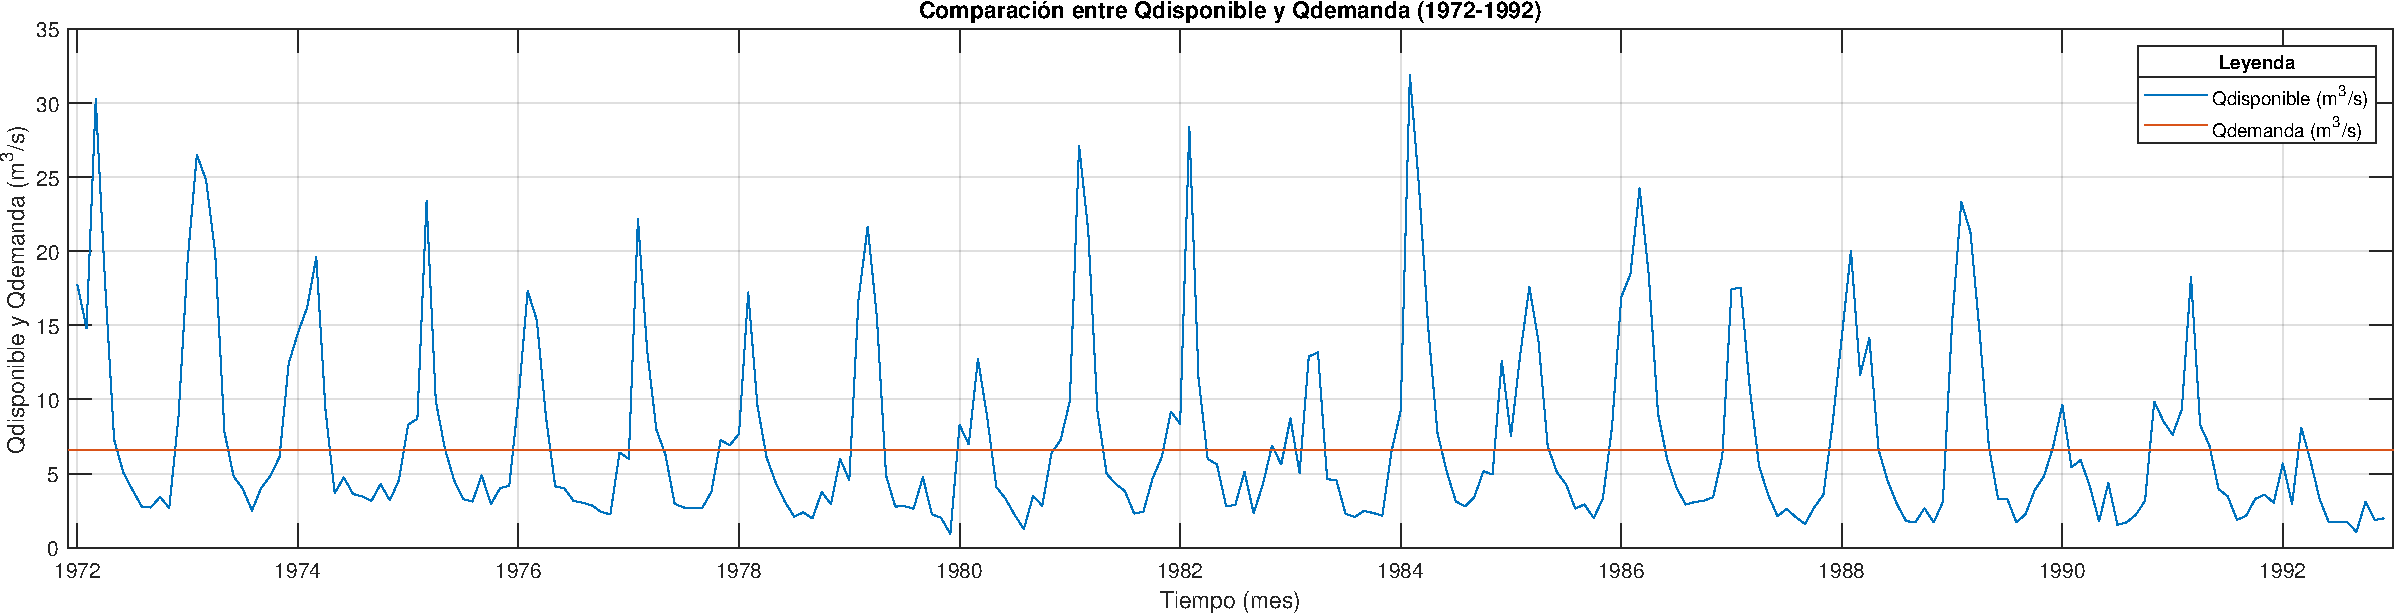
\includegraphics[width=0.7\textwidth]{Figures/Comparation.pdf}
        \captionsetup{labelfont=rm,skip=2pt,textfont=rm,font=small}
        \caption*{\textbf{FUENTE:} Elaboración propia}
    \label{fig:12}
\end{figure}

\begin{itemize}
    \item En la Figura \ref{fig:21}, se muestran los volúmenes medios mensuales acumulados de la estación Santa Eulalia (1972-1992).
\end{itemize}

\begin{figure}[H]
    \centering
    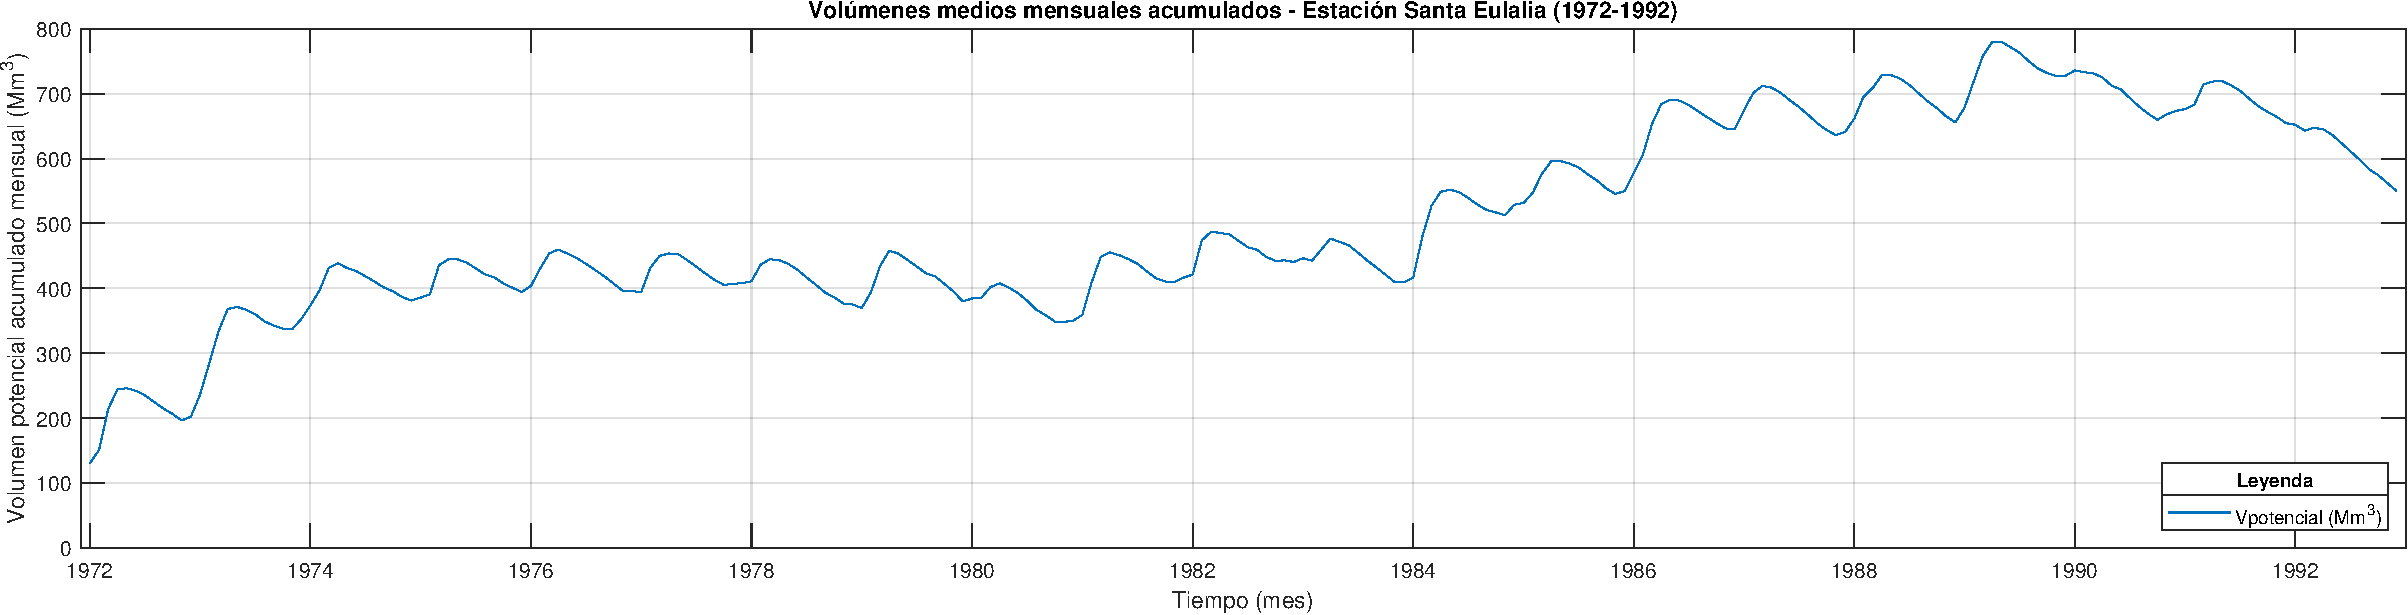
\includegraphics[width=0.7\textwidth]{Figures/Volumenes.pdf}
    \caption{Volúmenes medios mensuales acumulados}
    \captionsetup{labelfont=rm,skip=2pt,textfont=rm,font=small}
        \caption*{\textbf{FUENTE:} Servicio Nacional de Meteorología e Hidrología del Perú SENAMHI}
    \label{fig:21}
\end{figure}

\begin{table}[H]
\centering
  \begin{threeparttable}
    \caption{Sample ANOVA table}
     \begin{tabular}{lllll}
        \toprule \toprule
        Stubhead & \( df \) & \( f \) & \( \eta \) & \( p \) \\
        \midrule
                 &     \multicolumn{4}{c}{Spanning text}     \\
        Row 1    & 1        & 0.67    & 0.55       & 0.41    \\
        Row 2    & 2        & 0.02    & 0.01       & 0.39    \\
        Row 3    & 3        & 0.15    & 0.33       & 0.34    \\
        Row 4    & 4        & 1.00    & 0.76       & 0.54    \\
        \bottomrule
     \end{tabular}
    \begin{tablenotes}
    \vspace{-0.5cm}
        \item {{\fontsize{10pt}{ \baselineskip}\selectfont \textbf{FUENTE}: Elaboración propia}}
    \end{tablenotes}
\end{threeparttable}
\end{table}






\chapter{RESULTADOS Y DISCUSIÓN}
\thispagestyle{empty}
\begin{itemize}
    \item \lipsum[2]
    \item \lipsum[3]
\end{itemize}




\chapter{CONCLUSIONES}
\thispagestyle{empty}
\begin{enumerate}[leftmargin=1em]
    \item \lipsum[1]
    \item \lipsum[2]
    \item \lipsum[3]
    \item \lipsum[4]
\end{enumerate}

\chapter[\hspace{0.2cm}RECOMENDACIONES]{RECOMENDACIONES}
\thispagestyle{empty}

\begin{enumerate}[leftmargin=1em]
    \item \lipsum[3]
    \item \lipsum[2]
    \item \lipsum[5] \parencite{Niu2020}.
    \parencite{Niu2020} \parencite[see][p10]{Niu2020}\nptextcite{Niu2020} hola \textcite{Niu2020}
\end{enumerate}





\printbibliography[title={VII.\hspace{1em}REFERENCIAS BIBLIOGRÁFICAS}]
\addcontentsline{toc}{chapter}{VII. \textbf{REFERENCIAS BIBLIOGRÁFICAS}}
\thispagestyle{empty}

\appendix
\setcounter{chapter}{7}
\renewcommand{\thechapter}{\Roman{chapter}.}
\setcounter{section}{7}% Reset numbering for sections
\renewcommand{\thesection}{\arabic{chapter}.\arabic{section}}% Adjust

\chapter[\hspace{0.35cm}ANEXOS]{ANEXOS}
\thispagestyle{empty}
\section*{ANEXO 1: Mapas de la zona de estudio}\appcaption{ANEXO 1: Mapas de la zona de estudio}
...(contents of appendix one)...

\begin{figure}[htbp!]
    \centering
    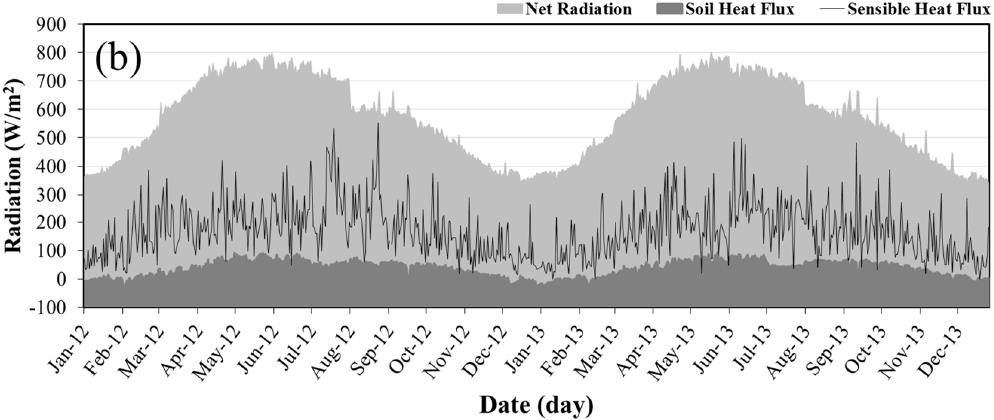
\includegraphics[width=0.9\textwidth]{Figures/f2.png}
    % \addto\captionsspanish{\renewcommand{\appendixname}{Anexo}}
    \caption*{Anexo 1.1: Variación temporal de los componentes del balance energético en la torre de flujo ubicada al centro de arrozales}
    \captionsetup{labelfont=rm,skip=2pt,textfont=rm,font=small}
        \caption*{\textbf{FUENTE:} \parencite{Lee2016}}
    \label{fig:a1}
\end{figure}

\section*{ANEXO 2: Mapas de la zona de estudio}\appcaption{ANEXO 2: Mapas de la zona de estudio}

\section*{ANEXO 3: Mapas de la zona de estudio}\appcaption{ANEXO 3: Mapas de la zona de estudio}


\end{document}
